%%%%%%%%%%%%%%%%%%%%%%%%%%%%%%%%%%%
%This is the LaTeX ARTICLE template for RSC journals
%Copyright The Royal Society of Chemistry 2016
%%%%%%%%%%%%%%%%%%%%%%%%%%%%%%%%%%%

\documentclass[twoside,twocolumn,9pt]{article}
\usepackage{extsizes}
\usepackage[super,sort&compress,comma]{natbib} 
\usepackage[version=3]{mhchem}
\usepackage[left=1.5cm, right=1.5cm, top=1.785cm, bottom=2.0cm]{geometry}
\usepackage{balance}
\usepackage{times,mathptmx}
\usepackage{sectsty}
\usepackage{graphicx} 
\usepackage{lastpage}
\usepackage[format=plain,justification=justified,singlelinecheck=false,font={stretch=1.125,small,sf},labelfont=bf,labelsep=space]{caption}
\usepackage{float}
\usepackage{fancyhdr}
\usepackage{fnpos}
\usepackage[english]{babel}
\usepackage{array}
\usepackage{droidsans}
\usepackage{charter}
\usepackage[T1]{fontenc}
\usepackage[usenames,dvipsnames]{xcolor}
\usepackage{setspace}
\usepackage[compact]{titlesec}
%%%Please don't disable any packages in the preamble, as this may cause the template to display incorrectly.%%%
\usepackage[obeyFinal]{easy-todo}
\usepackage{url}
\usepackage{rotating}


\usepackage{epstopdf}%This line makes .eps figures into .pdf - please comment out if not required.

\definecolor{cream}{RGB}{222,217,201}

\begin{document}

\pagestyle{fancy}
\thispagestyle{plain}
\fancypagestyle{plain}{

%%%HEADER%%%
\fancyhead[C]{
\includegraphics[width=18.5cm]{head_foot/header_bar}}
\fancyhead[L]{\hspace{0cm}\vspace{1.5cm}
\includegraphics[height=30pt]{head_foot/journal_name}}
\fancyhead[R]{\hspace{0cm}\vspace{1.7cm}
\includegraphics[height=55pt]{head_foot/RSC_LOGO_CMYK}}
\renewcommand{\headrulewidth}{0pt}
}
%%%END OF HEADER%%%

%%%PAGE SETUP - Please do not change any commands within this section%%%
\makeFNbottom
\makeatletter
\renewcommand\LARGE{\@setfontsize\LARGE{15pt}{17}}
\renewcommand\Large{\@setfontsize\Large{12pt}{14}}
\renewcommand\large{\@setfontsize\large{10pt}{12}}
\renewcommand\footnotesize{\@setfontsize\footnotesize{7pt}{10}}
\makeatother

\renewcommand{\thefootnote}{\fnsymbol{footnote}}
\renewcommand\footnoterule{\vspace*{1pt}% 
\color{cream}\hrule width 3.5in height 0.4pt \color{black}\vspace*{5pt}} 
\setcounter{secnumdepth}{5}

\makeatletter 
\renewcommand\@biblabel[1]{#1}            
\renewcommand\@makefntext[1]% 
{\noindent\makebox[0pt][r]{\@thefnmark\,}#1}
\makeatother 
\renewcommand{\figurename}{\small{Fig.}~}
\sectionfont{\sffamily\Large}
\subsectionfont{\normalsize}
\subsubsectionfont{\bf}
\setstretch{1.125} %In particular, please do not alter this line.
\setlength{\skip\footins}{0.8cm}
\setlength{\footnotesep}{0.25cm}
\setlength{\jot}{10pt}
\titlespacing*{\section}{0pt}{4pt}{4pt}
\titlespacing*{\subsection}{0pt}{15pt}{1pt}
%%%END OF PAGE SETUP%%%

%%%FOOTER%%%
\fancyfoot{}
\fancyfoot[LO,RE]{\vspace{-7.1pt}
\includegraphics[height=9pt]{head_foot/LF}}
\fancyfoot[CO]{\vspace{-7.1pt}\hspace{13.2cm}
\includegraphics{head_foot/RF}}
\fancyfoot[CE]{\vspace{-7.2pt}\hspace{-14.2cm}
\includegraphics{head_foot/RF}}
\fancyfoot[RO]{\footnotesize{\sffamily{1--\pageref{LastPage} ~\textbar  \hspace{2pt}\thepage}}}
\fancyfoot[LE]{\footnotesize{\sffamily{\thepage~\textbar\hspace{3.45cm} 1--\pageref{LastPage}}}}
\fancyhead{}
\renewcommand{\headrulewidth}{0pt} 
\renewcommand{\footrulewidth}{0pt}
\setlength{\arrayrulewidth}{1pt}
\setlength{\columnsep}{6.5mm}
\setlength\bibsep{1pt}
%%%END OF FOOTER%%%

%%%FIGURE SETUP - please do not change any commands within this section%%%
\makeatletter 
\newlength{\figrulesep} 
\setlength{\figrulesep}{0.5\textfloatsep} 

\newcommand{\topfigrule}{\vspace*{-1pt}% 
\noindent{\color{cream}\rule[-\figrulesep]{\columnwidth}{1.5pt}} }

\newcommand{\botfigrule}{\vspace*{-2pt}% 
\noindent{\color{cream}\rule[\figrulesep]{\columnwidth}{1.5pt}} }

\newcommand{\dblfigrule}{\vspace*{-1pt}% 
\noindent{\color{cream}\rule[-\figrulesep]{\textwidth}{1.5pt}} }

\makeatother
%%%END OF FIGURE SETUP%%%

%%%TITLE, AUTHORS AND ABSTRACT%%%
\twocolumn[
  \begin{@twocolumnfalse}
\vspace{3cm}
\sffamily
\begin{tabular}{m{4.5cm} p{13.5cm} }


\includegraphics{head_foot/DOI} & \noindent\LARGE{\textbf{Molecular electrometer and binding of cations to phospholipid bilayers$^\dag$}} \\%Article title goes here instead of the text "This is the title"
\vspace{0.3cm} & \vspace{0.3cm} \\

 & \noindent\large{Andrea Catte,\textit{$^{a\ddag}$} Mykhailo Girych,\textit{$^{b}$} Matti Javanainen,\textit{$^{c,d}$} Claire Loison,\textit{$^{e}$} Josef Melcr,\textit{$^{f}$} Markus S. Miettinen,\textit{$^{g,h}$} Luca Monticelli,\textit{$^{i}$} Jukka M{\"a}{\"a}tt{\"a},\textit{$^{j}$} Vasily S. Oganesyan,\textit{$^{a}$} O. H. Samuli Ollila,\textit{$^{\ast b}$} Joona Tynkkynen,\textit{$^{c}$} and Sergey Vilov,\textit{$^{e}$}
} \\%Author names go here instead of "Full name", etc.


\includegraphics{head_foot/dates} & \noindent\normalsize{
%The abstract should be a single paragraph which summarises the content of the article. Any references in the abstract should be written out in full \textit{e.g.}\ [Surname \textit{et al., Journal Title}, 2000, \textbf{35}, 3523].
Despite the vast amount of experimental and theoretical studies on the binding affinity of cations into phospholipid bilayers, 
especially the biologically relevant Na$^+$ and Ca$^{2+}$ ions,  there is no consensus in the literature. 
In this paper, we show that the ion binding affinity can be directly compared between simulations and experiments by 
using the choline headgroup order parameters according to the 'molecular electrometer' 
concept [Seelig \textit{et al., Biochemistry}, 1987, \textbf{26}, 7535].
Our findings strongly support the view that Na$^+$ and other monovalent ions
(except Li$^+$) do not specifically bind to phosphatidylcholine lipid bilayers with sub-molar concentrations, 
in contrast to Ca$^{2+}$ and other multivalent ions. Especially the Na$^+$ binding affinity is 
overestimated by several molecular dynamics simulation models, leading to 
an artificially positively charged lipid bilayer and exaggerated structural effects in the headgroups. 
Qualitatively correct headgroup order parameter response is observed with
Ca$^{2+}$ binding in all the tested models, however, none of the them has a sufficient 
quantitative accuracy to interpret the Ca$^{2+}$:lipid stoichiometry or the induced atomistic resolution structural changes.
This work has been done as a fully open collaboration, using \url{nmrlipids.blogspot.fi} as a main communication platform; 
all the scientific contributions were made publicly on this blog. } \\%The abstrast goes here instead of the text "The abstract should be..."

\end{tabular}

 \end{@twocolumnfalse} \vspace{0.6cm}

  ]
%%%END OF TITLE, AUTHORS AND ABSTRACT%%%

%%%FONT SETUP - please do not change any commands within this section
\renewcommand*\rmdefault{bch}\normalfont\upshape
\rmfamily
\section*{}
\vspace{-1cm}


%%%FOOTNOTES%%%

\footnotetext{\textit{$^{a}$~School of Chemistry, University of East Anglia, Norwich, NR4 7TJ, United Kingdom}}
\footnotetext{\textit{$^{b}$~Department of Neuroscience and Biomedical Engineering, Aalto University, Espoo, Finland}}
\footnotetext{\textit{$^{c}$~Tampere University of Technology, Tampere, Finland}}
\footnotetext{\textit{$^{d}$~University of Helsinki, Helsinki, Finland}}
\footnotetext{\textit{$^{e}$~Univ Lyon, Universit{\'e} Claude Bernard Lyon 1, CNRS, Institut Lumi{\'e}re Mati{\'e}re, F-69622, LYON, France}}
\footnotetext{\textit{$^{f}$~Institute of Organic Chemistry and Biochemistry, Czech Academy of Sciences, Flemingovo n{\'a}m. 2, 16610 Prague 6, Czech Republic, Charles University in Prague, Faculty of Mathematics and Physics, Ke Karlovu 3, 121 16 Prague 2, Czech Republic}}
\footnotetext{\textit{$^{g}$~Fachbereich Physik, Freie Universit\"at Berlin, Berlin, Germany}}
\footnotetext{\textit{$^{h}$~Max Planck Institute of Colloids and Interfaces, Department of Theory and Bio-Systems, Potsdam, Germany}}
\footnotetext{\textit{$^{i}$~Institut de Biologie et Chimie des Prot{\'e}ines (IBCP), CNRS UMR 5086, Lyon, France}}
\footnotetext{\textit{$^{j}$~Aalto University, Espoo, Finland}}
\footnotetext{\textit{$^{\ast}${\bf Author to whom correspondence may be addressed. E-mail: samuli.ollila@aalto.fi.}}}


%\footnotetext{\textit{$^{b}$~Address, Address, Town, Country. Fax: XX XXXX XXXX; Tel: XX XXXX XXXX; E-mail: xxxx@aaa.bbb.ccc}} }}



%Please use \dag to cite the ESI in the main text of the article.
%If you article does not have ESI please remove the the \dag symbol from the title and the footnotetext below.
\footnotetext{\dag~Electronic Supplementary Information (ESI) available: %[details of any supplementary information available should be included here]. 
5 figures, detailed technical discussion and simulation details.
See DOI: 10.1039/b000000x/}
%additional addresses can be cited as above using the lower-case letters, c, d, e... If all authors are from the same address, no letter is required

\footnotetext{\ddag~The authors are listed in alphabetical order. 
%Additional footnotes to the title and authors can be included \textit{e.g.}\ `Present address:' 
%or `These authors contributed equally to this work' as above using the symbols: \ddag, \textsection, 
%and \P. Please place the appropriate symbol next to the author's name and include a \texttt{\textbackslash footnotetext} 
%entry in the the correct place in the list.
}


%%%END OF FOOTNOTES%%%

%%%MAIN TEXT%%%%


\section{Introduction}

Due to its high physiological importance --- nerve cell signalling being the prime example ---
interaction of cations with phospholipid membranes
has been widely studied via theory, simulations, and experiments.
The relative ion binding affinities are generally agreed to
follow the Hofmeister series~\cite{eisenberg79,cevc90,tocanne90,binder02,celma07,leontidis09,vacha09a,klasczyk10,harb13}, 
however,
consensus on the quantitative affinities is currently lacking.
Until 1990, the consensus (documented in two extensive reviews~\cite{cevc90,tocanne90}) was that
while  multivalent cations interact significantly with phospholipid bilayers,
for monovalent cations (with the exception of Li$^+$) the interactions are weak.
This conclusion has since been strengthened by further
studies showing that bilayer properties remain unaltered upon the addition of sub-molar concentrations of monovalent 
salt~\cite{binder02,pabst07,filippov09}.
Since 2000, however, another view has emerged, suggesting much stronger interactions between phospholipids and monovalent cations, and strong Na$^{+}$ binding in particular~\cite{bockmann03,bockmann04,vacha09a,manyes05,manyes06,fukuma07,leontidis09,ferber11,morata12,klasczyk10,harb13}.

The pre-2000 view has the experimental support that
(in contrast to the significant effects caused by any multivalent cations)
sub-molar concentrations of NaCl have a negligible effect on
phospholipid infrared spectra~\cite{binder02},
area per molecule~\cite{pabst07},
dipole potential~\cite{clarke99},
lateral diffusion~\cite{filippov09},
and choline head group order parameters~\cite{akutsu81};
in addition, the water sorption isotherm of a NaCl--phospholipid system
is highly similar to that of a  pure NaCl solution
--- indicating that the ion--lipid interaction is very weak~\cite{binder02}. 

The post-2000 'strong binding' view rests on experimental and above all simulation findings.
At sub-molar NaCl concentrations, the rotational and translational dynamics of membrane-embedded fluorescent probes decrease~\cite{bockmann03,vacha09a,harb13}, and atomic force microscopy (AFM) experiments show changes in bilayer hardness~\cite{manyes05,manyes06,fukuma07,ferber11,morata12};
in atomistic molecular dynamics (MD) simulations, phospholipid bilayers consistently bind Na${^+}$,
although the binding strength depends on the model used~\cite{bockmann03,bockmann04,sachs04,berkowitz06,cordomi08,cordomi09,valley11,berkowitz12}.

Some observables have been interpreted in favour of both views. For example,
as the effect of monovalent ions (except Li$^+$)  on the phase transition temperature is tiny
(compared to the effect of multivalent ions), it was initially interpreted 
as an indication that only multivalent ions and Li$^+$ specifically bind to phospholipid bilayers~\cite{cevc90}; 
however, such a small effect in calorimetric measurements was later interpreted to indicate that also
Na$^+$ binds~\cite{bockmann03,klasczyk10}.
Similarly, the lack of significant positive electrophoretic mobility
of phosphatidylcholine (PC) vesicles in the presence of NaCl
(again in contrast to multivalent ions and Li$^+$)
suggested weak binding of Na$^+$~\cite{eisenberg79,tatulian87,manyes05,manyes06,klasczyk10};
%NaCl increases the (initially negative) zeta potential to only about zero,
%whereas positive zeta potentials are generally reached with
however, these data have also been explained by a countering effect of the Cl$^-$ ions~\cite{berkowitz06,knecht13}.
To reduce the area per lipid in scattering experiments, molar concentrations of NaCl are required~\cite{pabst07}, which indicates weak ion--lipid interaction;
in MD simulations, however, already orders of magnitude lower concentrations result in Na$^+$ binding and clear reduction of area per lipid~\cite{bockmann03,cordomi08}.
Finally,  in noninvasive NMR experiments, lipid lateral diffusion is unaltered by NaCl~\cite{filippov09};
%suggesting that the fluorescence results arise from Na$^{+}$ interactions with probes rather than with lipids.
%This is pointed out in Conclusions, which I think is the best place for it. -markus.
however, it is reduced in simulations upon Na$^+$ binding,
which supports interpreting the reduced lateral diffusion of fluorescent probes~\cite{bockmann03,vacha09a,harb13}
as favouring the post-2000 view.

In this paper we set out to solve the apparent contradictions
between the pre-2000 and post-2000 views.
To this end we employ the 'molecular electrometer' concept,
according to which the changes in the order parameters of the $\alpha$ and $\beta$ carbons 
in the phospholipid head group (see Fig. \ref{POPCstructure}) can be used to measure the ion affinity to 
PC lipid bilayer~\cite{akutsu81,altenbach84,seelig87,scherer89}.
As order parameters can be accurately measured in experiments and directly compared to 
simulations \cite{ollila16}, employing the molecular electrometer as a function of cation concentration allows the 
comparison of binding affinity between simulations and experiments.
In addition to demonstrating the usefulness of this general concept,
we show that the response of order parameters to penetrating cations
is qualitatively correct in MD simulations, but that in several  models the affinity of Na$^{+}$ for PC bilayers
is grossly overestimated.
Moreover, we show that the accuracy of lipid--Ca$^{2+}$ interactions 
in current models is not enough for atomistic resolution interpretation of NMR experiments. 

This work has been done as an Open Collaboration at \url{nmrlipids.blogspot.fi};
all the related files \cite{githubIONpaper} %(\url{https://github.com/NMRLipids/lipid_ionINTERACTION})
and almost all the simulation data (\url{https://zenodo.org/collection/user-nmrlipids})
are openly available.

\begin{figure}[]
  \centering
  \includegraphics[width=8.6cm]{../Fig/POPCstructure.eps}

  \caption{\label{POPCstructure}
    Chemical structure of 1-palmitoyl-2-oleoylphosphatidylcholine (POPC), and the definition of $\gamma$, $\beta$, $\alpha$, $g_1$, $g_2$ and $g_3$ segments.}
  
\end{figure}


\section{Results and Discussion}

\subsection{Background: Molecular electrometer in experiments}\label{conceptinexperiments}
The molecular electrometer concept is based on the experimental observation that
binding of any charged objects (e.g. ions, peptides, anesthetics, amphihiles) on a PC bilayer interface induces 
systematic changes in the choline $\beta$ and $\alpha$
segment order parameters~\cite{akutsu81,altenbach84,altenbach85,seelig87,macdonald87,scherer89,roux90,beschiasvili91,marassi92,rydall92}.
Thus, these changes can be used to determine binding affinities of the charged objects.
The molecular electrometer was originally devised for cations~\cite{akutsu81,altenbach84}, but
further experimental quantification with various positively and negatively charged 
molecules showed that the choline order parameters $S_\mathrm{CH}^\alpha$ and $S_\mathrm{CH}^\beta$ 
in general vary linearly with small amount of bound charge per 
lipid~\cite{altenbach84,altenbach85,seelig87,macdonald87,scherer89,roux90,beschiasvili91,marassi92,rydall92}. 
The empirically observed linear relation can be written as~\cite{ferreira16}
\begin{equation}\label{electrometer_eq}
S_{\rm{CH}}^{i}(X^\pm)=S_{\rm{CH}}^{i}(0) + \frac{4m_i}{3\chi} X^\pm,
\end{equation}
where $S_{\rm{CH}}^{i}(0)$ is the order parameter in the absence of bound charges,
$m_i$ is an empirical constant depending on the valency and position of bound charge,
$X^\pm$ is the amount of the bound charge per lipid, 
$i$ refers to either $\alpha$ or $\beta$, and
the value of quadrupole coupling constant is $\chi \approx$ 167 kHz. 
The change in order parameters with respect to a bilayer without bound charges then becomes
\begin{equation}\label{OPchangeEQ}
\Delta S_{\rm{CH}}^{i}= S_{\rm{CH}}^{i}(X^\pm)-S_{\rm{CH}}^{i}(0) =\frac{4m_i }{3\chi}X^\pm.
\end{equation}
For Ca$^{2+}$ binding to POPC bilayer (in the presence of 100~mM NaCl),
combination of atomic absorption spectra and $^2$H NMR experiments gave
$m_\alpha=-20.5$  and $m_\beta=-10.0$~\cite{altenbach84}.

\begin{figure*}[t]
  \centering
  \includegraphics[width=15cm]{../Fig/OrderParameterIONSchanges.eps}
  \caption{\label{ordPions}
    The order parameter changes for $\beta$ and $\alpha$ segments as a function of NaCl (left column) 
    and CaCl$_2$ (right column) concentration, from simulations and experiments~\cite{akutsu81} 
    (POPC with CaCl$_2$ from \cite{altenbach84}). The signs of the experimental order parameters, taken from
    experiments without ions~\cite{hong95a,hong95b,gross97}, can be assumed to be unchanged 
    with concentrations represented here~\cite{altenbach84,ollila16}. 
    It should be noted that none of the models used here reproduces the order parameters
    within experimental error for pure PC bilayer without ions, indicating structural inaccuracies with varying severity in all
    models \cite{botan15}. Note that the relatively large decrease in CHARMM36 with 450~mM CaCl$_2$ arise from more equilibrated binding 
    affinity due to long simulation times, see ESI$^\dag$.
  }
\end{figure*}

The absolute values of order parameters 
increase for $\beta$ and decrease for $\alpha$ segment with bound positive charge
and {\it vice versa} for negative charge~\cite{akutsu81,altenbach84,altenbach85,seelig87,scherer89,rydall92}. 
However, as the $\beta$ carbon order parameter is negative while $\alpha$ carbon order parameter is 
positive~\cite{hong95a,hong95b,gross97}, we can conclude 
that both $\Delta S_{\rm{CH}}^{\beta}$ and $\Delta S_{\rm{CH}}^{\alpha}$ decrease with bound positive charge 
and increase with bound negative charge. Consequently, values of $m_i$ are negative for
bound positive charges and {\it vice versa}. This can be rationalised by electrostatically 
induced changes in choline P--N dipole tilt \cite{seelig87,scherer89,seelig90}, which is also
seen in simulations~\cite{gurtovenko05,cordomi08,cordomi09,zhao12}. 
This is in line with order parameter decrease related to the P--N vector tilting more parallel to membrane plane seen with decreasing hydration levels~\cite{botan15}. 


The quantification of $\Delta S_\mathrm{CH}^\beta$ and $\Delta S_\mathrm{CH}^\alpha$
with different cations
have revealed that $\Delta S_{\rm{CH}}^{\beta}/\Delta S_{\rm{CH}}^{\alpha} \approx$ 0.5 for a wide range
of different cations (aqueous cations, cationic peptides, cationic anesthetics)~\cite{beschiasvili91,rydall92}.
More specifically,
the relation $\Delta S_{\rm{CH}}^{\beta}=0.43 \Delta S_{\rm{CH}}^{\alpha}$ was found for a DPPC bilayer
with various CaCl$_2$ concentrations~\cite{akutsu81}.


\subsection{Molecular electrometer concept in MD simulations}\label{electrometerinsimulations}

The headgroup order parameter changes as a function of ion concentration in
solution from H$^2$ NMR experiments are shown in Fig.~\ref{ordPions} for DPPC and POPC bilayers~\cite{akutsu81,altenbach84}.
Only minor changes in order parameters are seen
as a function of NaCl in solution, 
while the effect of CaCl$_2$ is an order of magnitude larger. 
Thus, according to the molecular electrometer concept, 
monovalent Na$^+$ ions have negligible affinity for PC lipid bilayers at concentrations up to 1 M,
while binding of Ca$^{2+}$ ions at the same concentration is significant~\cite{akutsu81,altenbach84}. 
%({\it Note that in contrast to the response as a function of bound charge in 
%Eq.~\eqref{electrometer_eq}, the changes in Fig.~\ref{ordPions}
%are not linear. This can be explained by electrostatic repulsion between
%already bound calcium ions and ions in solution \cite{altenbach84}.}
%\todo{Is this really needed? The x-axis of Fig.~\ref{ordPions} is not $X^\pm$, so
%why would one even expect the curves to follow Eq.~\eqref{electrometer_eq}?})
%SAMULI: I have removed this now.


Figure~\ref{ordPions} also reports order parameter changes calculated from MD simulations
of DPPC and POPC lipid bilayers as a function of NaCl or CaCl$_2$ initial concentrations in solution
(for details of the simulated systems see Tables~\ref{IONsystems},~\ref{IONsystems2} and ESI$^\dag$).
Note that none of these MD models
reproduced within experimental uncertainty the order parameters for a pure PC bilayer without ions
(Figure 2 in Ref.~\citenum{botan15}),
indicating structural inaccuracies of varying severity in all models \cite{botan15}.
However, the experimentally observed headgroup order parameter increase with dehydration
was qualitatively reproduced by all the models \cite{botan15}, and 
similarly here the presence of cations leads to the decrease 
of $S_\mathrm{CH}^\beta$ and $S_\mathrm{CH}^\alpha$ (Fig. \ref{ordPions}), in qualitative
agreement with experiments. The changes are, however, overestimated by most models.
According to the electrometer concept this indicates overbinding of cations in most MD simulation
models.

While electrometer concept is well established in experiments (see previous section),
it is not {\it a priori} clear that it works in simulations. The overestimated order parameter
decrease could, in principle, arise also from the oversensitivity of choline headgroups on cation binding,
instead of overbinding. Here we analyse the relation between cation binding and choline order 
parameter decrease in simulations in order to evaluate the usability of the electrometer concept in MD simulations.

According to the molecular electrometer concept, order parameter changes are linearly proportional to
the amount of bound cations in bilayer (Eq.~\eqref{OPchangeEQ}).
Figure~\ref{electrometer} shows the changes in order parameter as a function of bound charge in MD simulations
(see ESI$^\dag$ for the definition of bound ions);
in keeping with the molecular electrometer, roughly linear correlation between bound charge and order parameter change is found in all models.
Note that quantitative comparison of the proportionality constants (i.e. slopes in Fig. \ref{electrometer})
between different models and experimental slopes
($m_\alpha=-20.5$ and $m_\beta=-10.0$ for Ca$^{2+}$ binding in DPPC bilayer in
the presence of 100mM NaCl in Eq. \ref{electrometer_eq}~\cite{altenbach84}) is not straightforward 
since the simulation slopes depend on the definition used for bound ions (see ESI$^\dag$).
% -- \todo{put the definition of bound charges to ESI}). 
% This is already in the other todo point.
\begin{figure}[t]
  \centering
  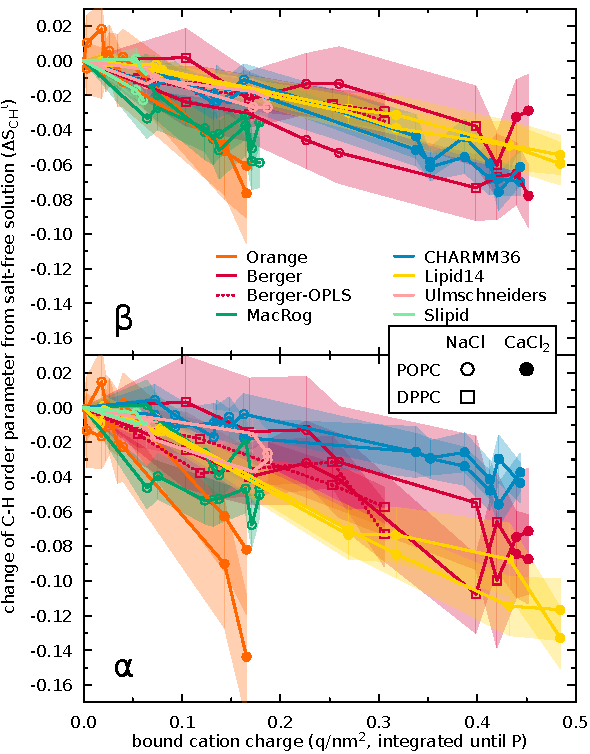
\includegraphics[width=8.6cm]{../scratch/boundIons/dOP_vs_boundCationCharge_P.pdf}
  \caption{\label{electrometer}
    Change of order parameters (from salt-free solution) of the $\beta$ and $\alpha$ segments,
    $\Delta S_{\rm{CH}}^{\beta}$ and $\Delta S_{\rm{CH}}^{\alpha}$,
    shown as a function of bound cation charge.
    Eight MD simulation models compared.
    The order parameters as well as the bound charge calculated separately for
    each leaflet; cations residing between the bilayer centre and the density maximum of Phosphorus
    considered bound; error bars show standard error of mean over lipids.
   }
%\todo{Results from long CHARMM and Slipids simulations to be added.}
\end{figure}

The comparison of order parameter changes in response to bound charge is more straightforward for
systems with charged amphiphiles fully associated in bilayer, as the amount of bound charge
is then explicitly known in both simulations and experiments. Such comparison
between previously published simulation data \cite{miettinen09} and experiments \cite{scherer89,franzin98}
could not rule out
overestimation of order parameter response to bound cations (i.e., slopes $m_\beta$ and $m_\alpha$)
in a Berger-based model (ESI$^\dag$).
This might, in principle, explain the overestimated order parameter 
response of Berger model to CaCl$_2$, but not to NaCl (see discussion in ESI$^\dag$).
Since simulation data with charged amphiphiles from other models is not available,
the extended comparison with different models is left for further studies.

Figure~\ref{electrometer} shows that the decrease on order parameter clearly correlates with the
amount of bound cations also in simulations. This is also evident from Fig.~\ref{NAdensities},
which shows the Na$^+$ density profiles of the MD models
ordered according to the order parameter change 
(reported in Fig.~\ref{ordPions}) from the smallest (top) to the largest (bottom).
The Na$^+$ density peaks are larger for models with larger changes in order parameters,
in line with the observed correlation between cation binding and order parameter decrease in
Fig.~\ref{electrometer}.
\begin{figure}[t]
  \centering
  \includegraphics[width=8cm]{../Fig/NAdensities.eps}
  \caption{\label{NAdensities}
    Atom number density profiles along the membrane normal for lipids, Na$^+$, and Cl$^-$ ions 
    from simulations with different force fields and different NaCl concentrations. 
    The force fields are ordered according to the order parameter changes 
    reported in Fig.~\ref{ordPions}, from the smallest (top panel) to the largest (bottom panel).
    The lipid densities are scaled by 100 (united atom) or 200 (all atom model) to improve readability. 
%    Figure discussed in https://github.com/NMRLipids/lipid\_ionINTERACTION/issues/4.
}
\end{figure}

Figure~\ref{AvsB} compares the relation between $\Delta S_{\rm{CH}}^{\beta}$ and $\Delta S_{\rm{CH}}^{\alpha}$
in experiments~\cite{akutsu81} and different simulation models.
Only Lipid14 gives $\Delta S_{\rm{CH}}^{\beta}/\Delta S_{\rm{CH}}^{\alpha}$ ratio in agreement with the experimental ratio.
In all the other models the $\alpha$ order parameter decrease with bound cations is underestimated with
respect to $\beta$ order parameter decrease.
\begin{figure}[t]
  \centering
  \includegraphics[width=8cm]{../Fig/OrderParameterAvsB.eps}
  \caption{\label{AvsB}
    Relation between $\Delta S_{\rm{CH}}^{\beta}$ and $\Delta S_{\rm{CH}}^{\alpha}$ from experiments~\cite{akutsu81} and
    different simulation models. Solid line is $\Delta S_{\rm{CH}}^{\beta}=0.43\Delta S_{\rm{CH}}^{\alpha}$ determined for DPPC bilayer
    from $^2$H NMR experiment with various CaCl$_2$ concentrations~\cite{akutsu81}.
  }
\end{figure}




In conclusion, the clear correlation between bound cations and order parameter decrease 
is observed in all the tested simulation models. Consequently, the electrometer concept can 
be used to compare the cation binding affinity between experiments and simulations. 
However, we find that the quantitative response of $\alpha$ and $\beta$ segment order parameters to bound cations in simulations 
do not generally agree with the experiments. The $\Delta S_{\rm{CH}}^{\beta}/\Delta S_{\rm{CH}}^{\alpha}$ ratio  
agrees with experiments only in Lipid14 model (Fig.~\ref{AvsB}). 
Thus, the observed overestimation of the order parameter changes with cation concentrations may, in principle, arise
from overbinding of ions or from too sensitive lipid headgroup response on bound cation 
(see also discussion in ESI$^\dag$). 
A careful analysis with current lipid models is performed in the next section.

\begin{sidewaystable*}[!p]
\centering
\caption{List of simulations performed in this work. The ion concentrations are calculated as 
   [ion]=(N$_{\rm ion} \times$[water])/N$_{\rm w}$, where [water]=55.5M. 
   These correspond the concentrations reported in the experiments by Akutsu et al.~\cite{akutsu81}.
   The lipid force fields are named as in our previous work~\cite{botan15}.}\label{IONsystems}
\begin{tabular}{c c c c c c c c c c c c}
  %\hline
  % some footnotes are not visible in typeset-MS (pdf)
  Force field (lipid, ion)& lipid & [Ion] mM & \footnote{The number of lipid molecules}N$_{\rm l}$   &  \footnote{The number of water molecules}N$_{\rm w}$   & \footnote{The number of Na$^+$ molecules}N$_{\rm Na}$  & \footnote{The number of Ca$^{2+}$ molecules}N$_{\rm Ca}$   &  \footnote{The number of Cl molecules}N$_{\rm Cl}$ & \footnote{Simulation temperature}T (K)  & \footnote{The total simulation time}t$_{{\rm sim}}$(ns) & \footnote{Time frames used in the analysis}t$_{{\rm anal}}$ (ns) & \footnote{Reference for simulation files}Files\\
  \hline
  Berger-POPC-07\cite{ollila07a}   &   POPC & 0          & 128 & 7290 & 0  & 0  & 0 & 298  & 270 & 240 & \citenum{bergerFILESpopc}  \\
  Berger-POPC-07\cite{ollila07a}, ffgmx\cite{straatsma88}  &   POPC & 340 (NaCl) & 128 & 7202 & 44  & 0  & 44 &298  & 110 & 50 & \citenum{bergerPOPC340mMNaClfiles} \\
  %\hdashline
  Berger-POPC-07\cite{ollila07a}, ffgmx\cite{straatsma88}  &   POPC & 340 (CaCl$_2$) & 128 & 7157 & 0 & 44  & 88 &298 & 108 & 58 &\citenum{bergerPOPC340mMCaClfiles}  \\
  \hline
  Berger-DPPC-97\cite{marrink98}   &   DPPC & 0 & 72 & 2880 & 0  & 0  & 0 &323  & 60 & 50 &\citenum{bergerDPPCfiles} \\
  Berger-DPPC-97\cite{marrink98}, ffgmx\cite{straatsma88}   &   DPPC & 150 (NaCl) & 72 & 2880 & 8  & 0  & 8 &323  & 120 & 60 &\citenum{bergerDPPC150mMfiles} \\
  Berger-DPPC-97\cite{marrink98}, ffgmx\cite{straatsma88}   &   DPPC & 1000 (NaCl) & 72 & 2778 & 51  & 0  & 51 &323  & 120 & 60 &\citenum{bergerDPPC1000mMfiles} \\
  \hline
  BergerOPLS-DPPC-06\cite{tieleman06} &   DPPC & 0 & 72 & 2880 & 0  & 0  & 0 &323  & 120 & 60 &\citenum{bergerOPLSDPPCfiles} \\
  BergerOPLS-DPPC-06\cite{tieleman06}, OPLS\cite{aqvist90} &   DPPC & 150 (NaCl) & 72 & 2880 & 8  & 0  & 8 &323  & 120 & 60 &\citenum{bergerOPLSDPPCfiles150mMnacl} \\
  BergerOPLS-DPPC-06\cite{tieleman06}, OPLS\cite{aqvist90} &   DPPC & 1000 (NaCl) & 72 & 2778 & 51  & 0  & 51 &323  & 120 & 60 &\citenum{bergerOPLSDPPCfiles1000mMnacl} \\
  \hline
  CHARMM36\cite{klauda10}   & POPC & 0           & 72 & 2242 & 0  & 0 & 0 & 303  & 30 & 20 & \citenum{charmm36filesSHORT} \\
  CHARMM36\cite{klauda10}, CHARMM36\cite{venable13} & POPC & 350 (NaCl)  & 72 & 2085 & 13  & 0 & 13 & 303  & 80 & 60 & \citenum{charmmPOPC350mMNaClfiles} \\
  CHARMM36\cite{klauda10}, CHARMM36\cite{venable13} & POPC & 690 (NaCl)  & 72 & 2085 & 26  & 0 & 26 & 303  & 73 & 60 & \citenum{charmmPOPC690mMNaClfiles}   \\
  CHARMM36\cite{klauda10}, CHARMM36\cite{venable13}  & POPC & 950 (NaCl)  & 72 & 2168 & 37  & 0 & 37 & 303  & 80 & 60 &\citenum{charmmPOPC950mMNaClfiles}  \\
  CHARMM36\cite{klauda10}, CHARMM36 & POPC &  350 (CaCl$_2$)  & 128 & 6400 & 0& 35 & 70 & 303  & 200  & 100 & \citenum{charmmPOPC350mMCaClfiles}  \\
  CHARMM36\cite{klauda10}, CHARMM36 & POPC &  450 (CaCl$_2$)  & 200 & 9000 & 0& 73 & 146 & 310  & 2000  & 100 & \citenum{charmmPOPC450mMCaClfiles}  \\
  CHARMM36\cite{klauda10}, CHARMM36 & POPC &  670 (CaCl$_2$)  & 128 & 6400 & 0& 67 & 134 & 303  & 200  & 120 & \citenum{charmmPOPC670mMCaClfiles}  \\  
  CHARMM36\cite{klauda10}, CHARMM36 & POPC &  1000 (CaCl$_2$) & 128 & 6400 & 0& 100 & 200 & 303 & 200  & 100 & \citenum{charmmPOPC1000mMCaClfiles}  \\
  \hline
  CHARMM36\cite{klauda10}, Yoo\cite{yoo16}  & DPPC & 430 (CaCl$_2$)  & 128 & 7760 & 0 & 60  & 120 & 323  & 200 & 170 & -  \\
  CHARMM36\cite{klauda10}, Yoo\cite{yoo16}  & DPPC & 886 (CaCl$_2$)  & 128 & 7520 & 0 & 120 & 240 & 323  & 200 & 170 & -  \\
  \hline
  MacRog\cite{maciejewski14}  & POPC & 0 & 288 & 14400 & 0 & 0 & 0 & 310 & 90&40  &~\citenum{macrogdehydFILES}  \\
  MacRog\cite{maciejewski14}, OPLS\cite{aqvist90}  & POPC & 100 (NaCl) & 288 & 14554 & 27 & 0 & 27 & 310 & 90&50  & \citenum{macrogIONfiles} \\
  MacRog\cite{maciejewski14}, OPLS\cite{aqvist90}  & POPC &  210 (NaCl) & 288 & 14500 & 54 & 0 & 54 & 310 & 90&50  &\citenum{macrogIONfiles}  \\
  MacRog\cite{maciejewski14}, OPLS\cite{aqvist90}  & POPC &   310 (NaCl) & 288 & 14446 & 81 & 0 & 81 & 310 & 90&50  & \citenum{macrogIONfiles} \\
  MacRog\cite{maciejewski14}, OPLS\cite{aqvist90}  & POPC &   420 (NaCl) & 288 & 14392 & 108 & 0 & 108 & 310 & 90& 50  & \citenum{macrogIONfiles}  \\
\end{tabular}
\end{sidewaystable*} 

\begin{sidewaystable*}[!p]
\centering
\caption{List of simulations performed in this work. The ion concentrations are calculated as 
   [ion]=(N$_{\rm ion} \times$[water])/N$_{\rm w}$, where [water]=55.5M. 
   These correspond the concentrations reported in the experiments by Akutsu et al.~\cite{akutsu81}.
   The lipid force fields are named as in our previous work~\cite{botan15}.}\label{IONsystems2}
\begin{tabular}{c c c c c c c c c c c c}
  %\hline
  % some footnotes are not visible in typeset-MS (pdf)
  Force field (lipid, ion)& lipid & [Ion] mM & \footnote{The number of lipid molecules}N$_{\rm l}$   &  \footnote{The number of water molecules}N$_{\rm w}$   & \footnote{The number of Na$^+$ molecules}N$_{\rm Na}$  & \footnote{The number of Ca$^{2+}$ molecules}N$_{\rm Ca}$   &  \footnote{The number of Cl molecules}N$_{\rm Cl}$ & \footnote{Simulation temperature}T (K)  & \footnote{The total simulation time}t$_{{\rm sim}}$(ns) & \footnote{Time frames used in the analysis}t$_{{\rm anal}}$ (ns) & \footnote{Reference for simulation files}Files\\
  \hline
  Orange, OPLS\cite{aqvist90}  &   POPC & 0 & 72 & 2880 & 0 & 0  & 0 & 298 & 60 & 50 & \citenum{orangePOPCfiles}  \\
  Orange, OPLS\cite{aqvist90} &   POPC & 140 (NaCl) & 72 & 2866 & 7 & 0  & 7 & 298 & 120 & 60 &\citenum{orangePOPC140mMNaClfiles}  \\
  Orange, OPLS\cite{aqvist90}  &   POPC & 510 (NaCl) & 72 & 2802 & 26 & 0  & 26 & 298 & 120 & 100 &\citenum{orangePOPC510mMNaClfiles}   \\
  Orange, OPLS\cite{aqvist90}  &   POPC & 1000 (NaCl) & 72 & 2780 & 50 & 0  & 50 & 298 & 120 & 80 & \citenum{orangePOPC1000mMNaClfiles} \\
  %\hdashline
  Orange, OPLS &   POPC & 510 (CaCl$_2$)  & 72 & 2802 & 0 & 26  & 52 & 298 & 120 & 60 & \citenum{orangePOPC510mMCaClfiles}  \\
  \hline
  Slipids\cite{jambeck12}   &   DPPC & 0 & 128 &3840 & 0 & 0  & 0 & 323 & 150 & 100 &~\citenum{slipidsFILES}  \\
  Slipids\cite{jambeck12}, AMBER\cite{beglov94,roux96} &   DPPC & 150 (NaCl)  & 600 & 18000 & 49 & 0  &  49 & 323 & 100 & 40 &-  \\
  Slipids\cite{jambeck12}, AMBER\cite{beglov94,roux96} &   DPPC & 850 (NaCl)  & 128 & 3726 &  57 & 0  &  57 & 323 & 105 & 100 & \citenum{slipidsFILESdppc}  \\
  \hline
  Slipids\cite{jambeck12b}   &   POPC & 0 & 128 & 5120 & 0 & 0  & 0 & 303 & 200 & 150 &~\citenum{slipidsFILESpopc}  \\
  Slipids\cite{jambeck12b}, AMBER\cite{smith94}  &  POPC & 130 (NaCl) & 200 & 9000 & 21 & 0  & 21 & 310 & 105 & 100 &~\citenum{slipidsFILESpopc130mMnaclSD}  \\
  Slipids\cite{jambeck12b}, AMBER\cite{aqvist90}  &  POPC & 450 (CaCl) & 200 & 9000  & 0 & 73  & 146 & 310 & 2000 & 100 &~\citenum{slipidsFILESpopc450mMcacl}  \\
  \hline
  Lipid14~\cite{dickson14}, AMBER\cite{aqvist90}  &   POPC & 0          & 128 & 5120 & 0 & 0  & 0 & 298 & 205 & 200 &~\citenum{lipid14POPC0mMNaClfiles}  \\
  Lipid14~\cite{dickson14}, AMBER\cite{aqvist90}   &   POPC & 150 (NaCl) & 128 & 5120 & 12 & 0 & 12 & 298 & 205 & 200 &~\citenum{lipid14POPC150mMNaClfiles}  \\
  Lipid14~\cite{dickson14}, AMBER\cite{aqvist90}   &   POPC & 1000 (NaCl) & 128 & 5120 & 77 & 0 & 77 & 298 & 205 & 200 &~\citenum{lipid14POPC1000mMNaClfiles}  \\
  Lipid14~\cite{dickson14}, AMBER\cite{aqvist90}   &   POPC & 350 (CaCl$_2$) & 128 & 6400 & 0 & 35 & 70 & 298 & 200 & 100 &~\citenum{lipid14POPC350mMCaClfiles}  \\
  Lipid14~\cite{dickson14}, AMBER\cite{aqvist90}   &   POPC & 1000 (CaCl$_2$) & 128 & 6400 & 0 & 100 & 200 & 298 & 200 & 100 &~\citenum{lipid14POPC1000mMCaClfiles}  \\
  \hline
  Ulmschneiders~\cite{Ulmschneider09}, OPLS\cite{aqvist90}       &   POPC & 0          & 128 & 5120 & 0 & 0  & 0 & 298.15 & 205 & 200 &~\citenum{ulmschneiderPOPC0mMNaClfiles}  \\
  Ulmschneiders~\cite{Ulmschneider09}, OPLS\cite{aqvist90}       &   POPC & 150 (NaCl) & 128 & 5120 & 12 & 0  & 12 & 298.15 & 205 & 200 &~\citenum{ulmschneiderPOPC150mMNaClfiles}  \\
  Ulmschneiders~\cite{Ulmschneider09}, OPLS\cite{aqvist90}       &   POPC & 1000 (NaCl) & 128 & 5120 & 77 & 0  & 77 & 298.15 & 205 & 200 &~\citenum{ulmschneiderPOPC1000mMNaClfiles}  \\
\end{tabular}
\end{sidewaystable*} 








\subsection{Cation binding in different simulation models}

The order parameter changes (Fig.~\ref{ordPions}) and density distributions (Fig.~\ref{NAdensities})
demonstrate significantly different Na$^+$ binding affinities in different simulation models.
The best agreement with experiments (lowest $\Delta S_\mathrm{CH}^\alpha$ and $\Delta S_\mathrm{CH}^\beta$) is observed for those models (Orange, CHARMM36, and Lipid14; see Fig.~\ref{ordPions}) that also predict the lowest Na$^+$ densities 
in the membrane proximity (Fig.~\ref{NAdensities}).
In all the other tested models, the choline order parameter 
responses to NaCl are clearly overestimated (Fig.~\ref{ordPions}),
and the strength of the overestimation is clearly linked to the strength of the
Na$^+$ binding affinity (compare Figs.~\ref{ordPions} and~\ref{NAdensities});
this leads us to
conclude that sodium binding affinity is overestimated in all these models.


In the best three models, the order parameter changes with NaCl are small ($<0.02$), so
with the achieved statistical accuracy we cannot conclude 
which of the three has the most realistic Na$^+$ binding affinity,
especially at physiological NaCl concentrations ($\sim$ 150mM) 
relevant for most applications. 
The overestimated binding in the other models raise questions on the quality of the predictions from these models when NaCl is present.
%\todo{It has been suggested that we should add references here. The problem is that there are a lot of them and
%it is difficult to choose which ones to pick. Any opinions?} {\it Mention that there are many (hundreds?) of them in Web of Science? -markus.}
%OLLILA: I have left this like it is.
Especially interactions between charged molecules and lipid bilayer might be significantly
affected by the strong Na$^+$ binding, as it makes the bilayer effectively positively charged.

Significant Ca$^{2+}$ binding affinity to a phosphatidylcholine bilayer at sub-molar concentrations  
is agreed in the literature~\cite{akutsu81,altenbach84,cevc90,tocanne90}, however, several
details are yet under discussion. Simulations suggest that Ca$^{2+}$ bind to lipid carbonyl
oxygens with coordination number of 4.2~\cite{bockmann04}, while interpretation of NMR and 
scattering experiments suggest that one Ca$^{2+}$ interacts mainly with choline 
groups~\cite{hauser76,hauser78,herbette84} of two phospholipid molecules~\cite{altenbach84}. 
Simulation model correctly reproducing the order parameter changes would resolve the discussion
by giving atomistic resolution interpretation for the experiments.

As a function of CaCl$_2$ concentration, all but one (CHARMM36 with recent ion model by Yoo et al.~\cite{yoo16}),
model overestimate the order parameter decrease (Fig.~\ref{ordPions}). 
According to the molecular electrometer, this indicates overestimated Ca$^{2+}$ binding. 
This is the most likely scenario for the models where changes in both order parameters were overestimated,
however, in the case of CaCl$_2$ we cannot exclude the possibility that the headgroup response is oversensitive to
bound cations (see ESI$^\dag$).
In CHARMM36 with ion model by Yoo et al.~\cite{yoo16},
$\Delta S_\mathrm{CH}$ is overestimated for $\beta$  but underestimated for  $\alpha$,
in line with Fig.~\ref{AvsB} where $\Delta S_{\rm{CH}}^{\beta}/\Delta S_{\rm{CH}}^{\alpha}$ ratio
in CHARMM36 is larger  than in experiments. Since we do not know if $\Delta S_{\rm{CH}}^{\beta}$ or $\Delta S_{\rm{CH}}^{\alpha}$
is more realistic in CHARMM36, we cannot conclude if Ca$^{2+}$ binding is too strong or weak in this simulation model.
This could be resolved by comparing CHARMM36 model to the experimental data with known amount of bound charge 
(e.g., experiments with amphiphilic cations~\cite{scherer89,franzin98}), however, such simulation data are not
currently available.

The ion density distributions with CaCl$_2$ in Fig.~\ref{CAdensitiesCLEAR} show significant
Ca$^{2+}$ binding in all models, however, some differences occur in details.
The Berger model predicts deeper penetration depth (density maxima close to $\pm$1.8~nm) compared
to other models (density maxima close to $\pm$2~nm). The latter value is probably more realistic 
since $^1$H~NMR and neutron scattering data indicate that Ca$^{2+}$ interacts mainly with the 
choline group~\cite{hauser76,hauser78,herbette84,cevc90}. In CHARMM36, almost all Ca$^{2+}$
ions present in simulation bind in bilayer indicating strongest binding affinity among the tested
models. The difference is not as clear in Fig.~\ref{ordPions} because $\alpha$ carbon order parameters 
are the least sensitive to bound charge in CHARMM36 (Fig.~\ref{electrometer}).
\begin{figure}[t]
  \centering
  \includegraphics[width=8cm]{../Fig/CAdensitiesCLEAR.eps}
  \caption{\label{CAdensitiesCLEAR}
    Atom number density profiles along the membrane normal coordinate $z$ for lipids, Ca$^{2+}$ and Cl$^-$ ions from simulations 
    with different force fields.
    The profiles only with smallest available CaCl$_2$ concentration are shown for clarity.
    Figure including all the available concentrations is shown in ESI$^\dag$.
    The lipid densities are scaled with 100 (united atom) or 200 (all atom model) to make them visible with the used y-axis scale.
    The Cl$^-$ density is scaled with 2 to equalise charge density of ions.
%    Figure discussed in https://github.com/NMRLipids/lipid\_ionINTERACTION/issues/4.
  }
\end{figure}

The origin of inaccuracies in lipid--ion interactions and binding affinities in different models is far from clear.
Potential candidates could be, for example, discrepancies in the ion models~\cite{hess06,chen07,Reif13},
incomplete treatment of electronic polarizability~\cite{leontyev11}, or inaccuracies in the lipid headgroup 
description~\cite{botan15}. Cordomi et al.~\cite{cordomi09} showed that the Na$^+$ binding affinity decreases when ion radius increases
in the model, however, also the models with the largest radius show significant binding in DPPC bilayer simulated with
OPLS-AA force field~\cite{jorgensen96}. In our results, the Slipids model gives essentially similar binding affinity with 
ion parameters from Refs.~\citenum{smith94} and~\citenum{beglov94,roux96}. Further, the compensation of missing electronic 
polarizability by scaling ion charge~\cite{kohagen16,leontyev11} reduced Na$^+$ binding in Berger, 
BergerOPLS and Slipids models, but not enough to be in agreement with experiments (ESI$^\dag$). 
The charge-scaled Ca$^{2+}$ model~\cite{kohagen14} slightly reduced binding in CHARMM36, but did not have 
significant influence on binding in Slipids (ESI$^\dag$). Significant reduction of
Ca$^{2+}$ binding was observed with ion model by Yoo et al~\cite{yoo16}, however, the CHARMM36 lipid
model must be further analysed to fully interpret the results.

On the other hand, also the lipid models may have significant influence on ion binding behaviour.
For example, the same ion model and non-bonded parameters are used in the Orange and BergerOPLS~\cite{tieleman06} 
simulations, but while Na$^+$ ion binding affinity appears realistic in the Orange model, it is significantly overestimated 
in the BergerOPLS (Fig.~\ref{NAdensities}). However, realistic Na$^+$ binding does not directly relate
to realistic Ca$^{2+}$ binding (see Orange, Lipid14 and CHARMM36 in Fig.~\ref{ordPions}) or realistic choline
order parameter response to bound charge (see Orange and CHARMM36 in Fig.~\ref{AvsB}).
It should be also noted that the low binding affinity of Na$^+$ in CHARMM36 model is due to 
the additional repulsion added between sodium ions and lipid oxygens (NBFIX)~\cite{venable13} (ESI$^\dag$).
Altogether, our results indicate that probably both, lipid and ion force field parameters, need improvement to 
correctly predict the cation binding affinity, and the associated structural changes.


\section{Conclusions}
As suggested by the molecular electrometer concept~\cite{akutsu81,altenbach84,seelig87,scherer89},
the decrease in order parameters of $\alpha$ and $\beta$ carbons in the PC head group of lipids bilayers
is related to cation binding  in all tested simulation models (Fig.~\ref{electrometer}), despite of known inaccuracies 
in the actual atomistic resolution structures~\cite{botan15}. Hence the molecular electrometer concept allows a direct comparison
of Na$^+$ binding affinity between simulations and noninvasive NMR experiments.
The comparison reveals that most models overestimate Na$^+$ binding; only Orange, Lipid14, and CHARMM36 
predict realistic binding affinity. None of the tested models has the required accuracy to interpret
the Ca$^{2+}$:lipid stoichiometry or induced structural changes with atomistic resolution.

In general, our results support the pre-2000 view that at sub-molar concentrations, in contrast to Ca$^{2+}$ and other multivalent ions~\cite{eisenberg79,akutsu81,altenbach84,tatulian87,cevc90,tocanne90,clarke99,binder02,pabst07,filippov09},
Na$^+$ and other monovalent ions (except Li$^+$) do not specifically bind to phospholipid bilayers.
Concerning the interpretation of existing experimental data, our work supports Cevc's view~\cite{cevc90}
that the observed small shift in phase transition temperature is not indicative of Na$^+$ binding.
Further, our findings are in line with the noninvasive NMR spectroscopy work of Filippov et al.~\cite{filippov09} 
that proved the results of Refs.~\citenum{bockmann03,vacha09a,harb13} to be explainable by direct interactions between Na$^+$ ions and fluorescent probes.
Finally, as spectroscopic methods are in general more sensitive to atomistic details in fluid-like environment than AFM, our work indirectly suggests that the ion 
binding reported from AFM experiments on fluid-like lipid bilayer systems~\cite{manyes05,manyes06,fukuma07,ferber11,morata12} might be confounded with other physical features of the system.
%\todo{This feels like a detached comment\ldots Could we back this claim up, or rephrase? I mean, now it sounds a bit like we came to conclude based on our simulations that the AFM resolution is not enough. \\
%OLLILA: Rephrasing is welcomed. In the the end, my justification for this comment is that spectrocopy is in general more reliable for atomistic resolution information than AFM in fluid--like environment. Also, I think that the AFM data supporting Na binding is quite indirect and can be interpreted in many ways but full discussion about this would be quite complicated I think. }}
Concerning contradictions in MD simulation results, we reinterpret strong Na$^+$ binding as an artefact of several simulation models, e.g., the Berger model used in Refs.~\citenum{bockmann03,bockmann04}.

The artificial specific Na$^+$ binding in simulations may lead to doubtful results, since it effectively leads  to
positively charged phosphatidylcholine (PC) lipid bilayers even at physiological NaCl concentration.
Such a PC bilayer has distinctly different interactions with charged objects compared to a (more realistic)
model without specific Na$^+$ binding. Furthermore, the overestimation of Na$^+$ binding affinity may
extend also to other positively charged objects, say, membrane protein segments. This would affect
lipid--protein interactions and could explain, for example, contradicting results on electrostatic interactions 
between charged protein segments and lipid bilayer \cite{arkhipov13,kaszuba15}. In conclusion, 
more careful studies and model development on lipid bilayer--charged object interactions are
called for to make molecular dynamics simulations directly usable in a physiologically relevant
electrolytic environment. 
%I have changed back to ''directly usable'' because simulation can be used also for intepretation
%besides of prediction. Also I want to keep word directly because simulations might be usable
%but only with very careful analysis. 

% Seelig's 1987 paper where the concept molecular electrometer is first mentioned stresses that it is not limited to ion binding, but can be used to study "any process that modifies the electrical properties of the membrane surface". Maybe we should repeat that quote to emphasize that molecular electrometer is a general means to assess the membrane electrical responses. Currently many people use additional molecular probes to measure electric responses, yet the molecular electrometer is a "non-invasive, non-perturbing" alternative.

This work has been done as a fully open collaboration, using
\url{nmrlipids.blogspot.fi} as the communication platform. All the
scientific contributions have been communicated publicly through
this blog or GitHub repository \cite{githubIONpaper}.% \url{https://github.com/NMRLipids/lipid_ionINTERACTION}.
All the related content and data is available at Ref. \citenum{githubIONpaper}. %\url{https://github.com/NMRLipids/lipid_ionINTERACTION}.
%Befor publication I will create Zenodo link from GitHub repo which will be cited here.

%This work has been, and will be, progressed and discussed through the blog \url{nmrlipids.blogspot.fi}, through which 
%everyone is invited to join the discussion and make contributions. 
%The manuscript will be eventually submitted to an appropriate scientific journal. 
%Everyone who has contributed to the work through the blog will be offered 
%coauthorship. For more details see \url{nmrlipids.blogspot.fi}.   

{\bf Acknowledgements: }
AC and VSO wish to thank the Research Computing Service at UEA for access to the High Performance Computing Cluster. VSO acknowledges the Engineering and Physical Sciences Research Council in the UK for financial support (EP/L001322/1).
%
OHSO acknowledges Tiago Ferreira for very useful discussions, the Emil Aaltonen foundation for financial support, Aalto Science-IT project and CSC-IT Center for Science for computational resources. 
%
MSM acknowledges financial support from the Volkswagen Foundation (86110).
%
M.G. acknowledges financial support from Finnish Center of International Mobility (Fellowship TM-9363).
%
J. Melcr acknowledges computational resources provided by the CESNET LM2015042 and the CERIT Scientific Cloud LM2015085 projects under the program ''Projects of Large Research, Development, and Innovations Infrastructure''
%
LM acknowledges funding from the Institut National de la Sante et de la Recherche Medicale (INSERM).

\bibliography{refs} %You need to replace "rsc" on this line with the name of your .bib file
\bibliographystyle{rsc} %the RSC's .bst file


\end{document}
